\documentclass[tikz,border=8pt]{standalone}
\usepackage{tikz}
\usepackage{amsmath,amssymb}
\usetikzlibrary{arrows.meta,positioning,calc}

\begin{document}
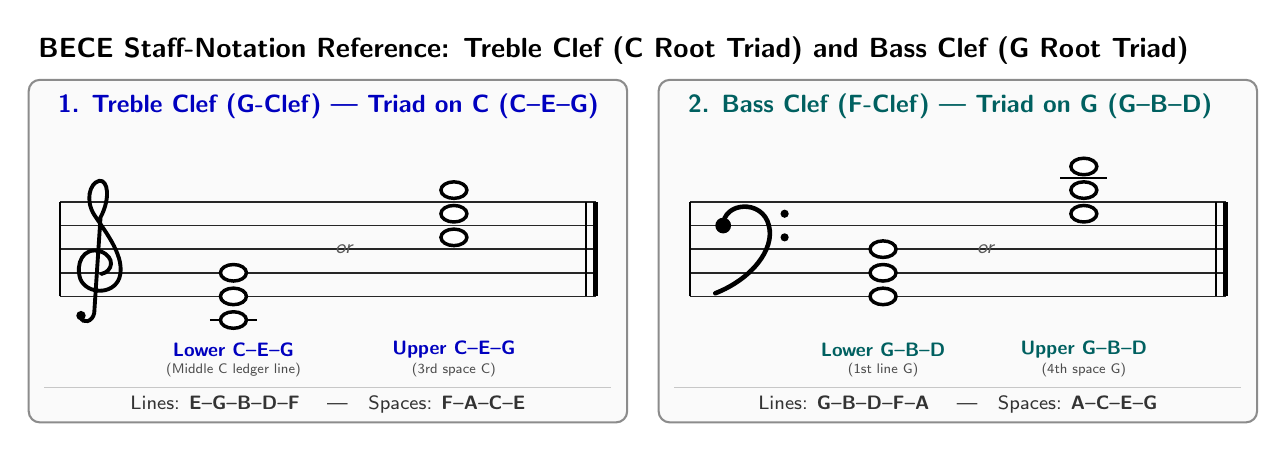
\begin{tikzpicture}[
    font=\sffamily,
    >=Stealth
]

\newcommand{\wholenote}[2]{%
    \fill[white] (#1, #2) ellipse (0.165 and 0.105);
    \draw[line width=1.25pt, black] (#1, #2) ellipse (0.165 and 0.105);
}

\node[font=\sffamily\bfseries\normalsize, anchor=west] at (0, 4.72)
    {BECE Staff-Notation Reference: Treble Clef (C Root Triad) and Bass Clef (G Root Triad)};

% =================== LEFT PANEL: TREBLE STAFF ===================
\draw[rounded corners=4pt, draw=black!45, fill=black!2, line width=0.75pt] (0, 0) rectangle (7.6, 4.35);
\node[font=\sffamily\bfseries\small, text=blue!75!black, anchor=west] at (0.25, 4.02)
    {1. Treble Clef (G-Clef) --- Triad on C (C--E--G)};

\begin{scope}[shift={(0.40, 1.60)}]
    % 5 lines: y = 0, 0.30, 0.60, 0.90, 1.20 (step = 0.15)
    \foreach \k in {0,1,2,3,4} {
        \draw[line width=0.6pt, black!85] (0, \k*0.30) -- (6.80, \k*0.30);
    }
    \draw[line width=0.8pt] (0, 0) -- (0, 1.20);
    \draw[line width=0.7pt] (6.68, 0) -- (6.68, 1.20);
    \draw[line width=1.9pt] (6.80, 0) -- (6.80, 1.20);

    % Treble Clef
    \begin{scope}[shift={(0.48, 0.30)}, scale=0.80]
        \draw[line width=1.4pt, black, line cap=round]
            (0.05, -0.02)
            .. controls (0.24, 0.02) and (0.28, 0.25) .. (0.04, 0.34)
            .. controls (-0.24, 0.42) and (-0.36, 0.14) .. (-0.28, -0.10)
            .. controls (-0.18, -0.34) and (0.24, -0.36) .. (0.34, -0.08)
            .. controls (0.44, 0.24) and (0.14, 0.62) .. (-0.06, 0.92)
            .. controls (-0.20, 1.14) and (-0.14, 1.42) .. (0.02, 1.46)
            .. controls (0.16, 1.48) and (0.20, 1.18) .. (0.04, 0.88)
            -- (-0.06, -0.64)
            .. controls (-0.09, -0.78) and (-0.24, -0.82) .. (-0.28, -0.70);
        \fill[black] (-0.27, -0.68) circle (0.075);
    \end{scope}

    % Position A: Lower C triad (C4 ledger = -0.30, E4 = 0.00, G4 = 0.30)
    \draw[line width=0.75pt] (1.90, -0.30) -- (2.50, -0.30);
    \wholenote{2.20}{-0.30}
    \wholenote{2.20}{0.00}
    \wholenote{2.20}{0.30}
    \node[font=\sffamily\scriptsize\bfseries, text=blue!75!black] at (2.20, -0.68) {Lower C--E--G};
    \node[font=\sffamily\tiny, text=black!70] at (2.20, -0.94) {(Middle C ledger line)};

    \node[font=\sffamily\scriptsize\itshape, text=black!65] at (3.60, 0.60) {or};

    % Position B: Upper C triad (C5 space 3 = 0.75, E5 space 4 = 1.05, G5 above line 5 = 1.35)
    \wholenote{5.00}{0.75}
    \wholenote{5.00}{1.05}
    \wholenote{5.00}{1.35}
    \node[font=\sffamily\scriptsize\bfseries, text=blue!75!black] at (5.00, -0.68) {Upper C--E--G};
    \node[font=\sffamily\tiny, text=black!70] at (5.00, -0.94) {(3rd space C)};
\end{scope}

% Dedicated bottom legend strip inside left panel
\draw[black!22, line width=0.45pt] (0.20, 0.44) -- (7.40, 0.44);
\node[font=\sffamily\scriptsize, text=black!80] at (3.80, 0.22)
    {Lines: \textbf{E--G--B--D--F} \quad|\quad Spaces: \textbf{F--A--C--E}};

% =================== RIGHT PANEL: BASS STAFF ===================
\draw[rounded corners=4pt, draw=black!45, fill=black!2, line width=0.75pt] (8.0, 0) rectangle (15.6, 4.35);
\node[font=\sffamily\bfseries\small, text=teal!75!black, anchor=west] at (8.25, 4.02)
    {2. Bass Clef (F-Clef) --- Triad on G (G--B--D)};

\begin{scope}[shift={(8.40, 1.60)}]
    % 5 lines: y = 0 (G2), 0.30 (B2), 0.60 (D3), 0.90 (F3), 1.20 (A3)
    \foreach \k in {0,1,2,3,4} {
        \draw[line width=0.6pt, black!85] (0, \k*0.30) -- (6.80, \k*0.30);
    }
    \draw[line width=0.8pt] (0, 0) -- (0, 1.20);
    \draw[line width=0.7pt] (6.68, 0) -- (6.68, 1.20);
    \draw[line width=1.9pt] (6.80, 0) -- (6.80, 1.20);

    % Bass Clef (F-clef) anchored on line 4 (F3 = 0.90)
    \begin{scope}[shift={(0.22, 0)}]
        \fill[black] (0.20, 0.90) circle (0.10);
        \draw[line width=1.65pt, black, line cap=round]
            (0.20, 0.90)
            .. controls (0.20, 1.20) and (0.70, 1.24) .. (0.78, 0.90)
            .. controls (0.86, 0.60) and (0.56, 0.22) .. (0.10, 0.04);
        \fill[black] (0.98, 1.05) circle (0.052);
        \fill[black] (0.98, 0.75) circle (0.052);
    \end{scope}

    % Position A: Lower G triad (G2 line 1 = 0.00, B2 line 2 = 0.30, D3 line 3 = 0.60)
    \wholenote{2.45}{0.00}
    \wholenote{2.45}{0.30}
    \wholenote{2.45}{0.60}
    \node[font=\sffamily\scriptsize\bfseries, text=teal!75!black] at (2.45, -0.68) {Lower G--B--D};
    \node[font=\sffamily\tiny, text=black!70] at (2.45, -0.94) {(1st line G)};

    \node[font=\sffamily\scriptsize\itshape, text=black!65] at (3.75, 0.60) {or};

    % Position B: Upper G triad (G3 space 4 = 1.05, B3 above line 5 = 1.35, D4 above C4 ledger = 1.65)
    \draw[line width=0.75pt] (4.70, 1.50) -- (5.30, 1.50); % Middle C ledger line above bass staff
    \wholenote{5.00}{1.05}
    \wholenote{5.00}{1.35}
    \wholenote{5.00}{1.65}
    \node[font=\sffamily\scriptsize\bfseries, text=teal!75!black] at (5.00, -0.68) {Upper G--B--D};
    \node[font=\sffamily\tiny, text=black!70] at (5.00, -0.94) {(4th space G)};
\end{scope}

% Dedicated bottom legend strip inside right panel
\draw[black!22, line width=0.45pt] (8.20, 0.44) -- (15.40, 0.44);
\node[font=\sffamily\scriptsize, text=black!80] at (11.80, 0.22)
    {Lines: \textbf{G--B--D--F--A} \quad|\quad Spaces: \textbf{A--C--E--G}};

\end{tikzpicture}
\end{document}
